\documentclass[12pt,oneside,a4paper]{article}

\usepackage[
  top=11em, 
  bottom=11em, 
  left=10em,
  right=10em]
  {geometry}

\usepackage{fancyhdr}
\lhead{\leftHeader}
\rhead{\rightHeader}
\renewcommand{\headrulewidth}{0pt}
\renewcommand{\footrulewidth}{0pt}

\hyphenation{ma-gyar}

\usepackage[hyphens]{url}

\usepackage{hyperref}
\usepackage[dvipsnames]{xcolor}
\hypersetup{
  colorlinks=true,
  urlcolor=MidnightBlue
}

\usepackage{fontspec}
\setmainfont[Mapping=tex-text,Numbers=OldStyle,Ligatures=TeX]{Linux Biolinum O}

\renewcommand{\baselinestretch}{1.1}

\usepackage{graphicx}
\graphicspath{{./}}
\usepackage{wrapfig}

\setlength{\parindent}{0em}

\def \leftHeader{CV}
\def \rightHeader{Simon Zsolt}

\setmainfont[Mapping=tex-text,Numbers=OldStyle,Ligatures=TeX]{TeX Gyre Termes}

\begin{document}

\begin{wrapfigure}{r}{13em}
  \flushright
  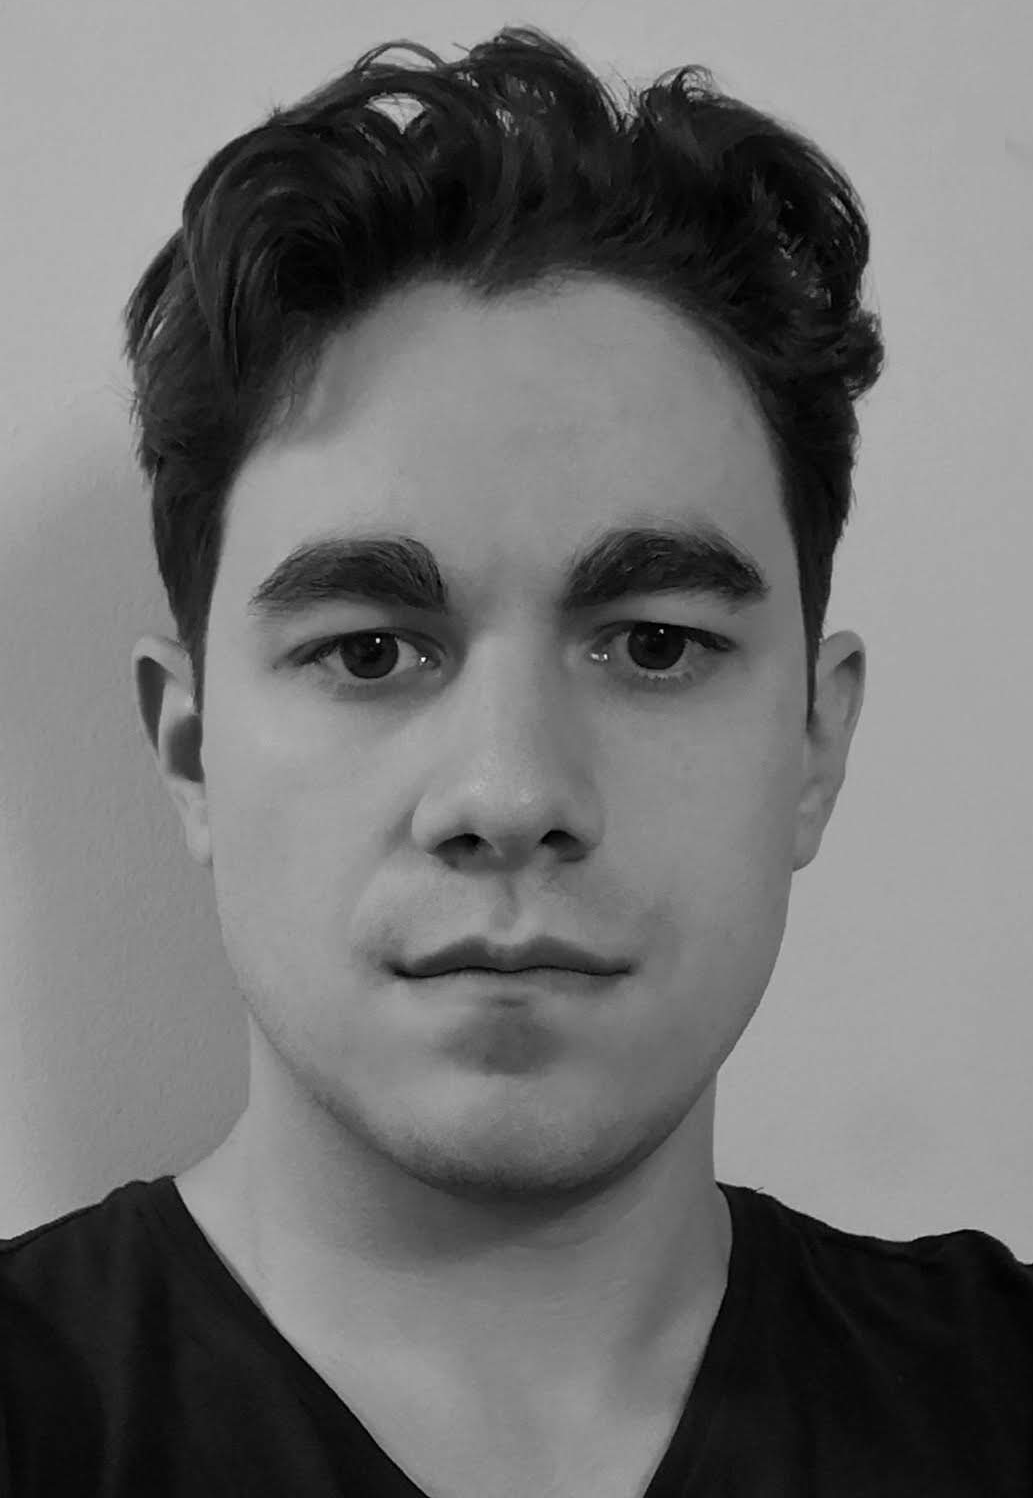
\includegraphics[scale=0.4]{portrait_mono} 
\end{wrapfigure}

\begin{Large}
  \textsc{Simon Zsolt}
  \vspace{1em}
\end{Large}

Születési dátum: 1989 Október 24\\
Cím: Magyarország, 2600, Vác,\\ \hspace*{1em} Erzsébet utca 10/A\\ 
GitHub: simonzsolt\\
E-mail: \url{simon.zsolt@mail.com}\\
Telefon: +36 20 4110 724

\vspace{1em}

Tanulmányok

\begin{itemize}
  \item{2015-től Eötvös Loránd Tudományegyetem Bölcsésztudományi Kar Reneszánsz Tanulmányok mesterszak}
  \item{2015: BA Eötvös Loránd Tudományegyetem Bölcsésztudományi Kar magyar alapképzési szak}
\end{itemize}

Tudományos és szakmai tevékenységek

\begin{itemize}
  \item{ 
    2017--2018: Javascript fejlesztő a Zeno Karl Schindler Alapítvány ösztöndíjas finanszírozásában, a SISMEL (Società Internazionale per lo Studio del Medioevo Latino) intézet megbízásából. 
    \url{http://www.sismelfirenze.it/index.php/formazione/borse-e-premi/item/219-mirabile-zeno-karl-schindler-foundation-fellowship-in-digital-humanities-2018} 
  }
  \item{2017-től közreműködő a  ``POSTDATA – Poetry Standardization and Linked
    Open Data'' projektben. }
  \item{2016 Október 17: Előadás a Pesti Bölcsész Akadémia konferenciasorozaton (ELTE)
    Gráfadatbázisok az irodalomtudományban címmel.\\
    \url{http://pestibolcseszakademia.blog.hu/2016/10/04/digitalis\_bolcseszet\_szovegen\_innen\_es\_tul\_marothy\_szilvia\_es\_simon\_zsolt\_kurzusa}
  }
  \item{2016 Október 24–28: DARIAH Winter School ``Open Data
    Citation for Social Science and Humanities'', Humanities at Scale project (HaS),
    Prága. }
  \item{2016 November 7: Előadás a Pesti Bölcsész Akadémia konferenciasorozaton (ELTE) Hálózati versadatbázisok címmel.\\
    \url{http://pestibolcseszakademia.blog.hu/2016/10/04/digitalis\_bolcseszet\_szovegen\_innen\_es\_tul\_marothy\_szilvia\_es\_simon\_zsolt\_kurzusa}
        }
  \item{2016 Február 1–6: Részvétel a ``Paleography, Codicology, Philology.
       Digital Editing of Medieval Manuscripts Training Programme'' képzésen.
       Klosterneuburg, Bécs. }
  \item{2015–2016: Technikai szerkesztője az Információtörténeti Műhely című sorozat alábbi megjelenéseinek: }
    \begin{itemize}
      \item{ \textsc{Bognár} Péter, \textit{A régi magyar párrímköltészet német vonatkozásai}, 2016,
        \url
         {htp://renaissance.elte.hu/wp-content/uploads/2016/02/parrim.pdf}
      }
      \item{ \textsc{Horváth} Iván, \textit{Ómagyar szövegemlékek mint textológiai tárgyak}, 2015,
        \url
         {http://renaissance.elte.hu/wp-content/uploads/2016/01/Omagyar\_szo\%CC\%88vegemle\%CC\%81kek\_d-ed-150bb.pdf}
      }
      \item{ \textsc{Tubay} Tiziano, \textit{A székely írás kutatásának története}, 2015,
        \url
         {http://renaissance.elte.hu/wp-content/uploads/2016/04/Tubay\_A-szekely-iras-kutatasanak-tortenete\_OSzK\_2015\_digitalis.pdf}
      }
    \end{itemize}
  \item{2015 November 24: Előadás a ``DHU2015 Workshop, Számító\-gép az
    irodalomtudományban'' című workshopon, az MTA BTK Irodalomtudományi Intézete és a BME Méréstechnikai és Információs Rendszerek Tanszéke közös szervezésével. 
    \url
     {htp://dhu2015.mit.bme.hu/felhivas} 
  }
  \item{2015: THECA – A középkori magyarországi könyvkatalógusok és könyvjegyzékek adatbázis fejlesztése.
    \url
     {http://hece.elte.hu/index.php/theca/}
  }
  \thispagestyle{fancy}
  \item{2015: A HECE -- Humanism in East Central Europe WordPress alapú blog szerkesztése. 
    \url
     {http://hece.elte.hu/}
  }
  \item{2014: Az Országos Széchényi Könyvtár Digitális Filológia osztályának korai közreműködője. 
    Az osztály hosszas szervezést követően nem alakult meg teljesen. }
  \item{2014: A Régi Magyar Exemplumadatbázis társ-fejlesztője és műszaki szerkesztője.
    \url
     {htp://sermones.elte.hu/exemplumadatbazis/}
  }
  \item{2013: A \textit{Mathias Rex 1458--1490: Hungary at the Dawn
         of the Renaissance} című kötet Junior szerkesztője.
    \url
     {http://renaissance.elte.hu/?page\_id=665} 
  }
  \item{2013--2016: Gyakornoki pozíció az ELTE BTK Magyar Irodalom-~és Kultúratudományi 
    Intézet Régi Magyar Irodalom Tanszékén.
  }
\end{itemize}

Szakmai ismeretek

  \begin{itemize}
    \item{Javascript: ES6, Node.js, Angular}
    \item{SQL és NoSQL adatbázisok: MariaDB, SQL Server, 
      MongoDB, OrientDB, ArangoDB, Elasticsearch, Neo4j}
    \item{git, JIRA}
    \item{UNIX-típusú rendszrek ismerete}
    \item{PHP, Perl, \LaTeX}
    \item{AWS, Heroku, OpenShift}
  \end{itemize}

Nyelvtudás
  
  \begin{itemize}
    \item{Angol: C1 komplex nyelvvizsga, folyékon szövegértés és fogalmazás}
    \item{Latin: alapszintű olvasási kompetencia}
    \item{Olasz: alapszintű olvasási és szövegértési kompetencia}
  \end{itemize}

\thispagestyle{fancy}

\end{document}